\documentclass[usenames,dvipsnames,t]{beamer}

\usepackage[orientation=portrait,size=a1,scale=1.4]{beamerposter}
\usepackage[utf8]{inputenc}
\usepackage{standalone}
\usepackage{amsmath}
\usepackage{amsfonts}
\usepackage{amsthm}
\usepackage{mathtools}
\usepackage{amssymb}
\usepackage{graphicx}
\usepackage{minted}
\usepackage{multicol}
\usepackage{tcolorbox}
\usepackage{tikz}
\usetikzlibrary{arrows}
\usetikzlibrary{decorations.markings}
\usetikzlibrary{decorations.text}
\usetikzlibrary{calc}
\usetikzlibrary{shapes.geometric}
\usetikzlibrary{patterns,snakes}
\usetikzlibrary{positioning}

\definecolor{textgrey}{HTML}{586e75}
\definecolor{textorange}{HTML}{cc5200}
\definecolor{ciwyellow}{HTML}{fbbe28}
\definecolor{mplblue}{HTML}{1339cd}
\definecolor{cream}{HTML}{fefff4}
\definecolor{newport}{HTML}{41B6af}
\definecolor{nowhere}{HTML}{42B929}
\definecolor{everywhere}{HTML}{cd2d89}

\setlength{\fboxrule}{2pt}

\setbeamercolor{structure}{fg=textorange}

\tikzset{
    partial ellipse/.style args={#1:#2:#3}{
        insert path={+ (#1:#3) arc (#1:#2:#3)}
    }
}

  \def\python{(0, 2) ellipse ({7.4} and {4})}
  \def\bestpractice{(-5, 0) ellipse ({4} and {6.4})}
  \def\opensource{(5, 0) ellipse ({4} and {6.4})}
  \def\documentation{(0, -2) ellipse ({7.4} and {4})}

\usemintedstyle{trac}

\beamertemplatenavigationsymbolsempty


\begin{document}

% Title
\begin{columns}
  \begin{column}{0.015\linewidth}
  \end{column}
  \begin{column}{0.11\linewidth}
    \begin{center}
      \vspace{2mm}
      
\includegraphics[width=\textwidth]{../cflogo}
    \end{center}
  \end{column}
  \begin{column}{0.575\linewidth}
    \begin{center}
      \vspace{3mm}
      \textcolor{textgrey}{\huge{CIW: AN OPEN-SOURCE DISCRETE-\\[5mm]EVENT-SIMULATION LIBRARY}}\\[10mm]
      \textcolor{textorange}{\LARGE{G.I. Palmer, V.A. Knight, P.R. Harper \& A.L. Hawa}}
      \vspace{5mm}
    \end{center}
  \end{column}
  \begin{column}{0.3\linewidth}
    \begin{center}
      \vspace{10mm}
      
\includegraphics[width=\textwidth]{../SSI_Logo}
    \end{center}
  \end{column}
  \begin{column}{0.015\linewidth}
  \end{column}
\end{columns}



\textcolor{textgrey}{\hrule height 3pt}

\vspace{5mm}
Reproducibility is the ``cornerstone of cumulative science''
(\textcolor{textorange}{Sandve et al. (2013)}), but many simulation software
fail in this aspect.
In \textcolor{textorange}{Kilgore (2001)} three properties of simualtion
software are identified as being vital for reproducibility:
\tcbox[boxrule=2pt, tcbox raise base, boxsep=-1mm, colback=ciwyellow!20, colframe=ciwyellow, arc=2mm, auto outer arc, nobeforeafter]{\textit{\!readability\!}},
\tcbox[boxrule=2pt, tcbox raise base, boxsep=-1mm, colback=mplblue!20, colframe=mplblue, arc=2mm, auto outer arc, nobeforeafter]{\textit{\!modularity\!}} and
\tcbox[boxrule=2pt, tcbox raise base, boxsep=-1mm, colback=textorange!20, colframe=textorange, arc=2mm, auto outer arc, nobeforeafter]{\textit{\!extendibility\!}}.
Ciw strives to accompish this:

\begin{columns}
\begin{column}{0.5\textwidth}
% \begin{center}
%   \textcolor{textgrey}{\Large{CIW \& REPRODUCIBILITY}\vspace{4mm}}
% \end{center}
\begin{center}
  \includestandalone[width=0.7\textwidth]{euler}

  \vspace{12mm}

  \begin{minipage}[c]{0.975\textwidth}
    \textbullet\ \textbf{Open-Source:} Software with source code that anyone can freely obtain, use, and modify.\\[3.5mm]
    \textbullet\ \textbf{Python:} A free open-source programming language that prioritises readability, with a well established   scientific ecosystem.\\[3.5mm]
    \textbullet\ \textbf{Documentation:} User guides, references and tutorials on how to use software and how the software works.\\[3.5mm]
    \textbullet\ \textbf{Best Practices:} Well written code incorporating readable and modular code, and automated tests.
  \end{minipage}
\end{center}

\vspace{5mm}
\textcolor{textgrey}{\hrule height 3pt}
\vspace{5mm}

\begin{center}
  \textcolor{textgrey}{\Large{PERFORMANCE}\vspace{4mm}}\\
  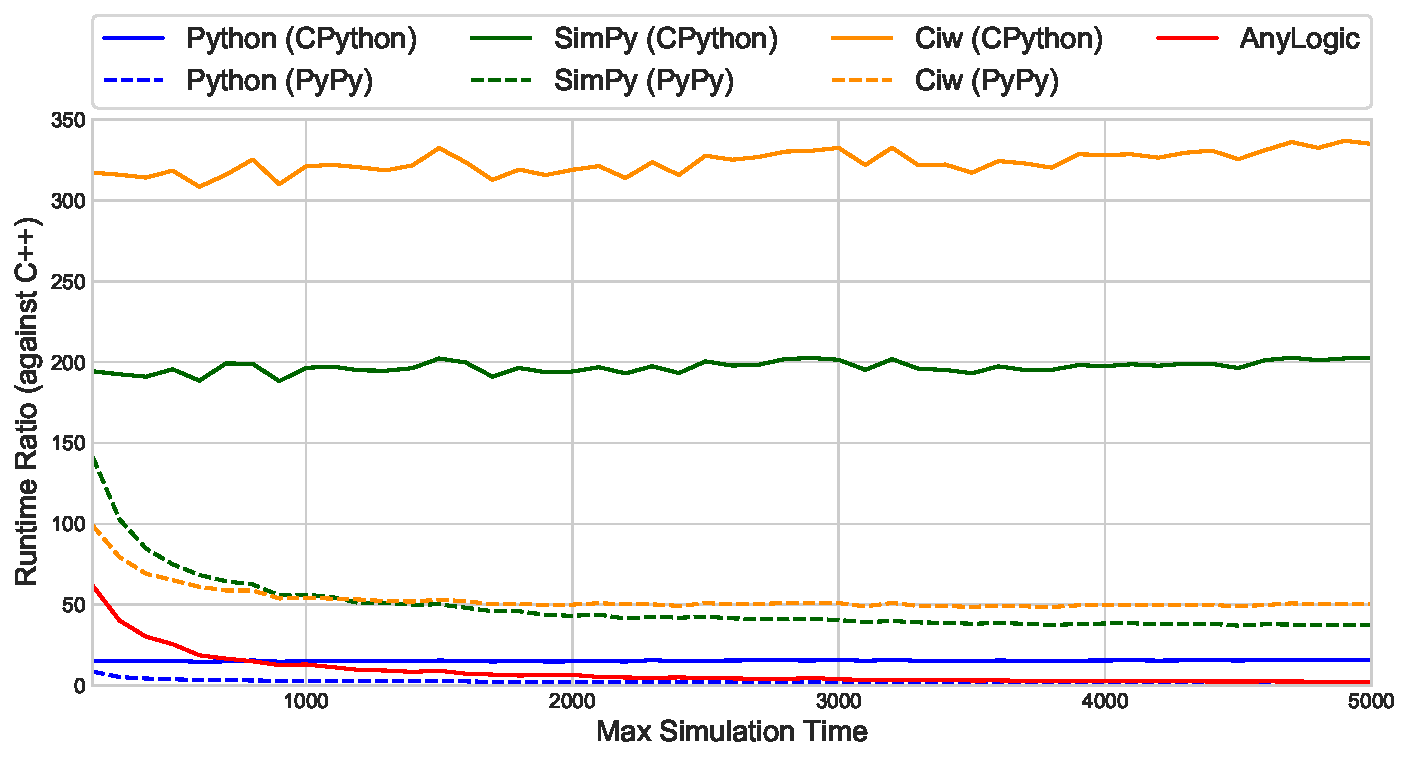
\includegraphics[width=0.7\textwidth]{runtimes}
\end{center}

\end{column}

\begin{column}{0.5\textwidth}
  \begin{center}
  \begin{minipage}[c]{0.9\textwidth}
    \begin{tcolorbox}[boxrule=2pt, colback=ciwyellow!15,colframe=ciwyellow, title=\small{READABLE}, coltitle=white, halign title=right]
      \begin{center}
        \small{
          \begin{minted}{python}
>>> import ciw
>>> N = ciw.create_network(
...     Arrival_distributions=[['Exponential', 10.0]],
...     Service_distributions=[['Exponential', 4.0]],
...     Number_of_servers=[3],
... )

>>> ciw.seed(0)
>>> Q = ciw.Simulation(N)
>>> Q.simulate_until_max_time(200)
>>> recs = Q.get_all_records()
>>> waits = [r.waiting_time for r in recs if r.arrival_date > 50]
>>> sum(waits) / len(waits)
0.3796...
          \end{minted}
        }
      \end{center}
    \end{tcolorbox}
    \vspace{10mm}
    \begin{tcolorbox}[boxrule=2pt, colback=mplblue!15,colframe=mplblue, title=\small{MODULAR}, coltitle=white, halign title=right]
          \begin{center}
            \includestandalone[width=\textwidth]{codestructure}
          \end{center}
          \small{
            \begin{minted}{python}
>>> Q
Simulation
>>> Q.nodes
[Arrival Node, Node 1, Exit Node]
>>> Q.nodes[1].all_individuals
[Individual 1941, Individual 1942, ...
>>> Q.nodes[1].all_individuals[0].service_time
0.8900655260040934
            \end{minted}
          }
    \end{tcolorbox}
    \vspace{10mm}
    \begin{tcolorbox}[boxrule=2pt, colback=textorange!15,colframe=textorange, title=\small{EXTENDIBLE}, coltitle=white, halign title=right]
    \begin{columns}
    \hspace{0.02\textwidth}
    \begin{column}{0.32\textwidth}
      \begin{center}
      \rotatebox{30}{\includestandalone[width=0.7\textwidth]{pricetag}}
      \end{center}
      \small{Open, permissive licence allows modifications.}
    \end{column}
    \begin{column}{0.32\textwidth}
      \begin{center}
      \includestandalone[width=0.6\textwidth]{puzzle}
      \end{center}
      \small{Modular structure enables contained adaptions and custom components.}
    \end{column}
    \begin{column}{0.32\textwidth}
      \begin{center}
      \includestandalone[width=0.95\textwidth]{fork}\\
      \end{center}
      \small{Systematic forking in GitHub gives opportuinty for changes to be released.}
    \end{column}
    \hspace{0.02\textwidth}
    \end{columns}
    \end{tcolorbox}
    \vspace{5mm}
  \end{minipage}
  \end{center}

\end{column}
\end{columns}

\vspace{12mm}
\textcolor{textgrey}{\hrule height 3pt}
\vspace{5mm}

\begin{center}
  \textcolor{textgrey}{\Large{A HEALTHCARE APPLICATION}\vspace{4mm}}
\end{center}

\begin{center}
\begin{minipage}{0.35\textwidth}
    \includestandalone[width=0.95\textwidth]{ophcn_map}
\end{minipage}
\hspace{3mm}
\begin{minipage}{0.25\textwidth}
  \textbullet\ Stay Well Plans (SWPs) offered to older people in Gwent.\\[2mm]
  \textbullet\ Ciw simulations used to evaluate their effects on system demand.\\[2mm]
  \textbullet\ Three scenarios compared:\\[0.5mm]
  \begin{tcolorbox}[boxrule=2pt, colback=nowhere!15,colframe=nowhere]
      SWPs not offered in Gwent.
  \end{tcolorbox}
  \begin{tcolorbox}[boxrule=2pt, colback=newport!15,colframe=newport]
      SWPs offered in Newport county only.
  \end{tcolorbox}
  \begin{tcolorbox}[boxrule=2pt, colback=everywhere!15,colframe=everywhere]
      SWPs offered in all counties of Gwent.
  \end{tcolorbox}
  \textbullet\ Inconsequential increases in demand at secondary care.\\[2mm]
  \textbullet\ Large increases in demand at home and day community care.\\[2mm]
  \textbullet\ Large decreases in demand at residential care services.
\end{minipage}
\hspace{3mm}
\begin{minipage}{0.35\textwidth}
    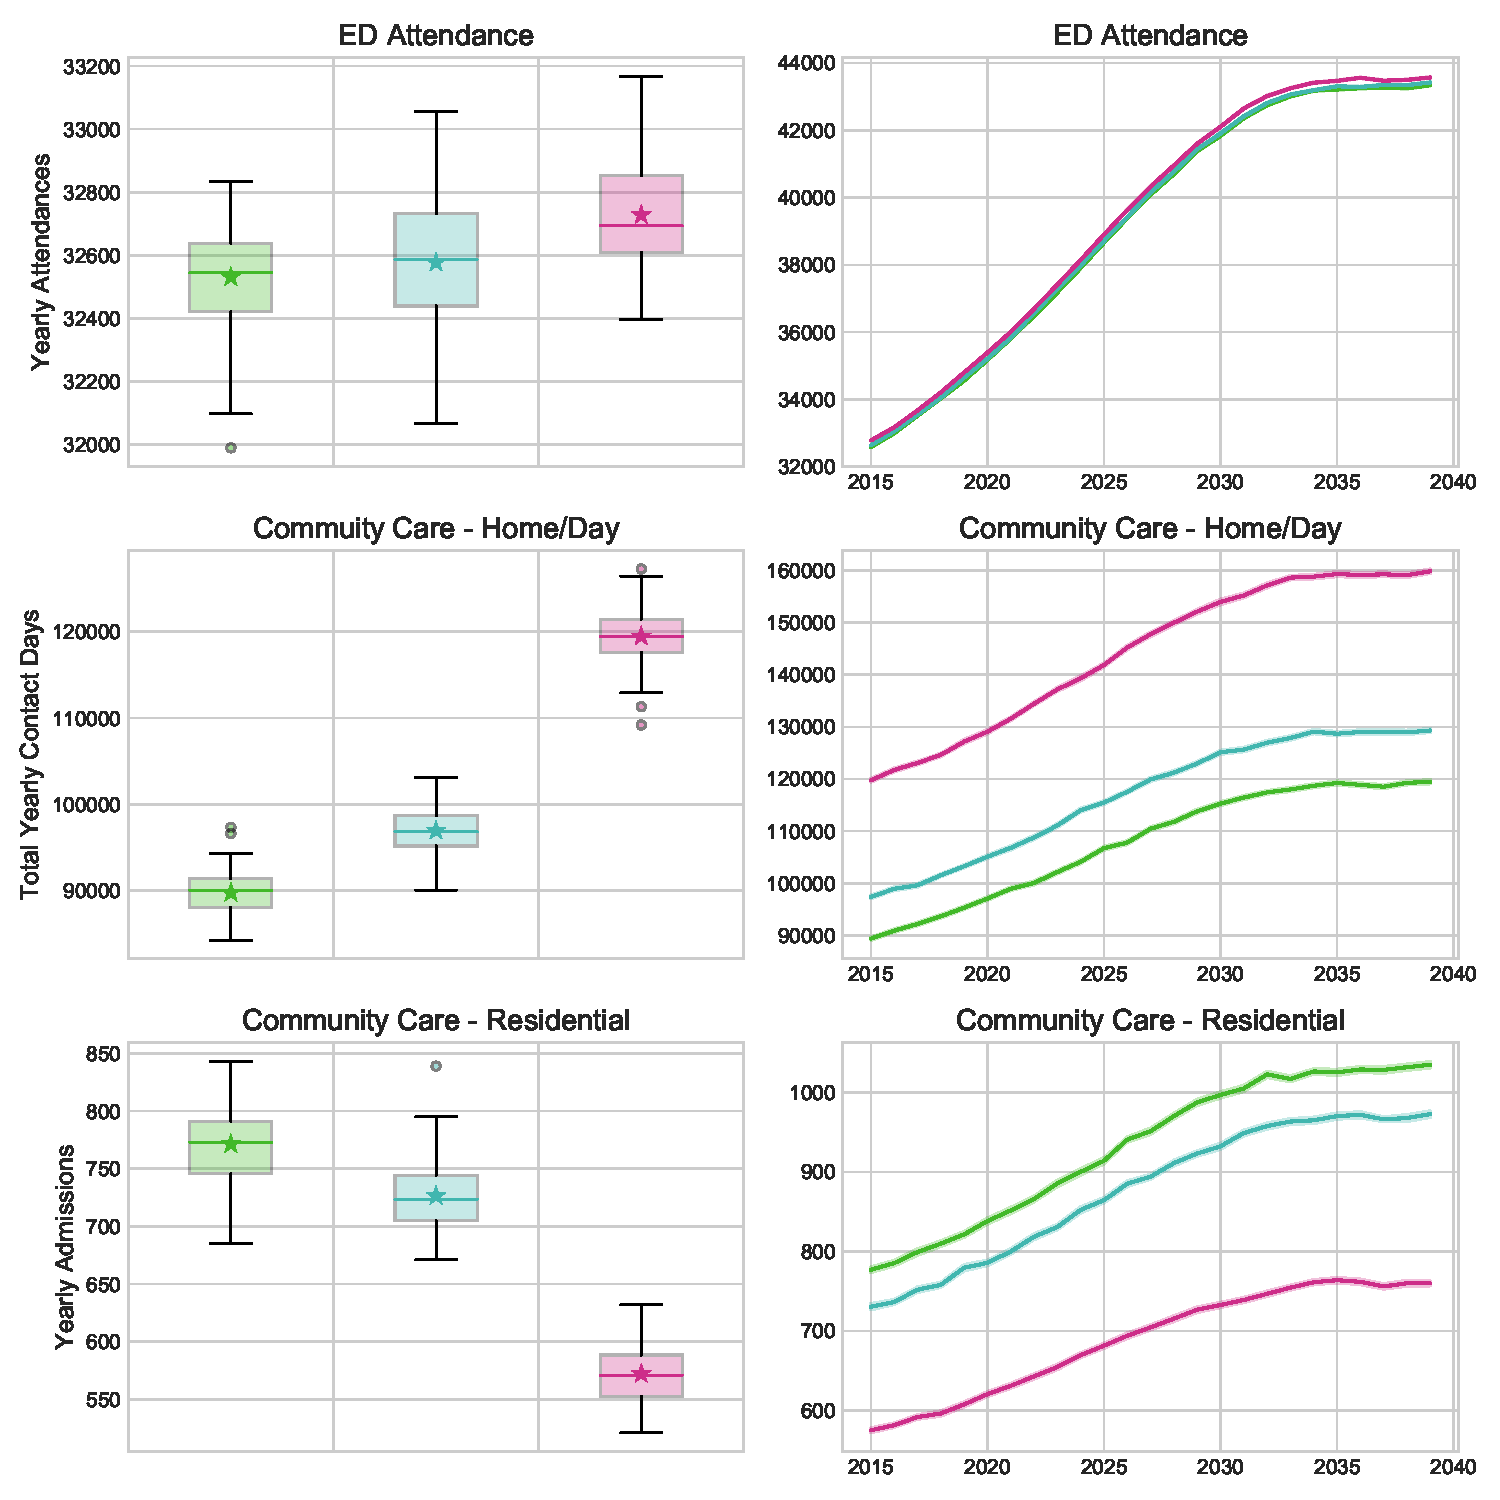
\includegraphics[width=\textwidth]{SWPplots}
\end{minipage}
\end{center}


\vspace{8mm}

\textcolor{textgrey}{\hrule height 3pt}

\vspace{4mm}

\begin{columns}
\begin{column}{0.88\textwidth}
\textcolor{textgrey}{\large{REFERENCES:}\vspace{2mm}}\\
\footnotesize{\textcolor{textorange}{
  \textbullet\ 2001: \textbf{Open source simulation modeling language (sml)}. Kilgore, RA. \textit{In Proceedings of the 33nd conference on Winter simulation (pp. 607–613). IEEE Computer Society}\\
  \textbullet\ 2013: \textbf{Ten simple rules for reproducible computational research}. Sandve, GK., Nekrutenko, A., Taylor, J., Hovig, E. \textit{PLoS Comutational Biology}\\
  \textbullet\ 2018: \textbf{Ciw: An open source discrete event simulation library}. Palmer GI, Knight VA, Harper PR, Hawa AL.\textit{Journal of simulation}.
}}\\[4mm]
\begin{center}
  \large{\texttt{https://github.com/CiwPython/Ciw} \hspace{80mm} \texttt{http://ciw.readthedocs.io/en/latest/}}
\end{center}
\end{column}
\begin{column}{0.1\textwidth}
  \begin{center}
  \vspace{-5mm}
  
\includegraphics[width=0.9\textwidth]{ciwlogo}
  \end{center}
\end{column}
\end{columns}

\end{document}